\section{Results and their interpretation}
\label{sec:results}

\subsection{A compact view of the frozen comparison}

Table~\ref{tab:overview} gives the aggregate result before the
instance-level analysis. A mean over an instance family gives each of
its fixed files equal weight. The planted exact-hit count is the number
of trial populations whose best final candidate reaches the planted
energy; it is not a count of all hitting replicas.

\begin{table*}[t]
\centering\small
\caption{Aggregate frozen endpoints. ``Best'' means largest final cut on
K2000 or smallest relative energy error on a planted instance. The
methods use their declared, unequal internal state budgets.}
\label{tab:overview}
\begin{tabular*}{\textwidth}{@{\extracolsep{\fill}}llrrr}
\toprule
Family & method & trials & mean & best; exact hits\\
\midrule
K2000 & \QeFEM{} & 5 & cut 33,281.2 & cut 33,293; gap 44\\
K2000 & \LQA{} & 5 & cut 33,249.0 & cut 33,249; gap 88\\
Wishart & \QeFEM{} & 50 & $\eps=4.0717\%$ & $0\%$; $7/50$\\
Wishart & \LQA{} & 50 & $\eps=6.9411\%$ & $2.0199\%$; $0/50$\\
Chook & \QeFEM{} & 110 & $\eps=0.2186\%$ & $0\%$; $60/110$\\
Chook & \LQA{} & 110 & $\eps=1.1086\%$ & $0\%$; $10/110$\\
\bottomrule
\end{tabular*}
\end{table*}

The aggregate advantage over this \LQA{} implementation is consistent
across the planted files, but the scale of that advantage depends on the
family and its parameter. The detailed plots and tables below show where
the exact hits arise. K2000 reveals a different pattern: a measurable
advantage over the saved \LQA{} endpoints, coupled to a persistent
44-unit shortfall against the stored cut reference.

\subsection{G-set: broad attainment with a measurable later gain}

The smooth-gradient study reached 23 of 54 supplied G-set reference cuts.
The later search on the remaining 31 produced ten additional matches,
for 33 cumulative matches. Eight of the ten new matches were recovered
after freezing a selected configuration and changing to the final
evaluation seeds: G15, G16, G18, G19, G21, G22, G24, and G25. G17 and
G28 were attained during search or promotion but not on their fresh
evaluation seeds. Among the 31 revisited graphs, the retained gap
decreased on 27.

\begin{figure*}[t]
\centering
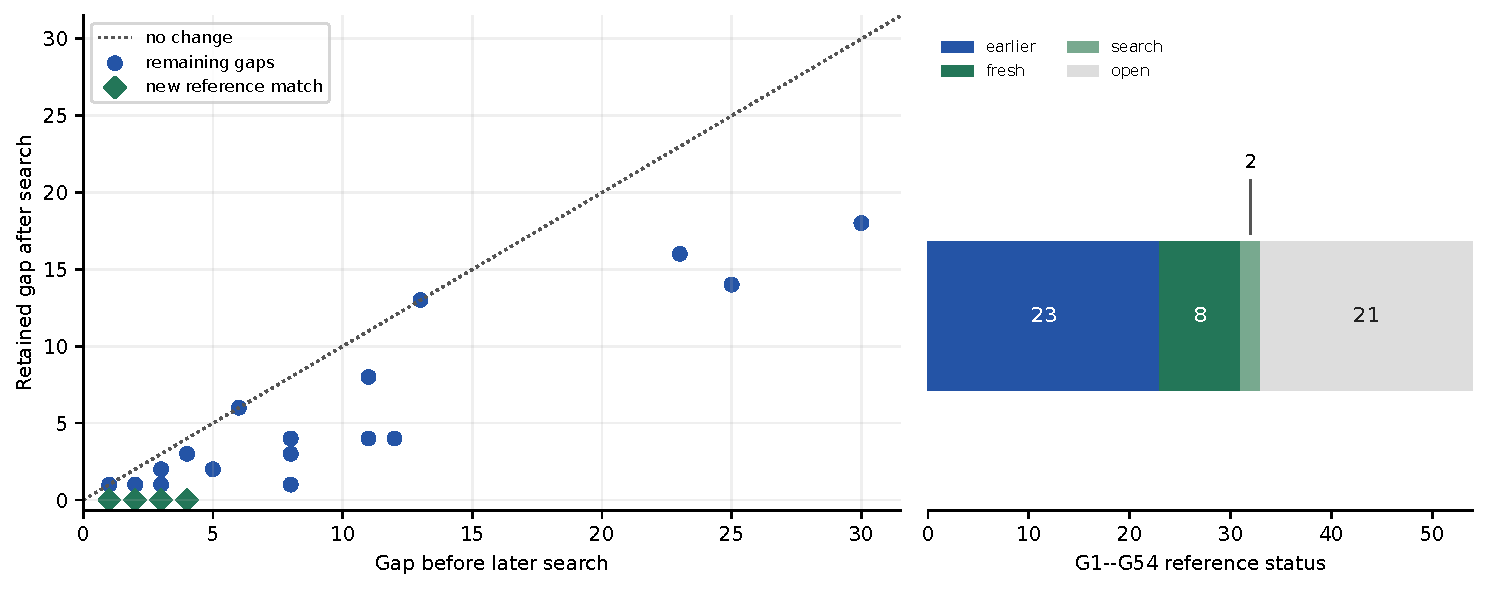
\includegraphics[width=\textwidth]{figures/gset_search_progress.pdf}
\caption{\textbf{Targeted \QeFEM{} updates extend
attainment on previously unresolved graphs.} Each point in the left panel
is one of the 31 graphs below its supplied reference before the later
search. Points below the diagonal improved; diamonds on the horizontal
axis are the ten new matches. The right panel separates the accumulated
54-graph inventory into 23 prior matches, eight new matches recovered
with fresh seeds, two found only during search, and 21 unmatched graphs.
Search budgets were adaptive, so the stacked bar is an attainment record,
not a universal success rate.}
\label{fig:gset-progress}
\end{figure*}

The improvements extend beyond the ten new matches. Most revisited
graphs move closer to their references even without reaching them. The
remaining failures are also concentrated: G14, G29, G30, G31, and G51
are one cut unit below their stored targets; G23, G26, and G40 are two
units below. The largest residuals are on G35--G38, with gaps 13, 16,
18, and 14 respectively. Appendix~\ref{app:fullresults} lists every
G1--G54 target, attained cut, gap, and evidence status. The 33 matches
do not establish an equal-budget advantage over another solver because
the cumulative search incorporated multiple graph-specific proposals.

\subsection{K2000: a strong cut, a population plateau, and an open gap}

K2000 tests a dense signed objective with nearly two million couplings.
The five frozen 8,192-replica \QeFEM{} trials yield cuts 33,274,
33,274, 33,274, 33,293, and 33,291. Their mean is 33,281.2 and sample
standard deviation is 9.88 cut units. The best cut is 44 below the
stored 33,337 reference, a residual of 0.132\% relative to that
reference. The corresponding five \LQA{} endpoints all equal 33,249,
giving gap 88. The smaller \QeFEM{} gap is an attainable-quality result
under these frozen method settings; it is not a matched-time win because
one \QeFEM{} trial evolves 8,192 states and one \LQA{} trial evolves one.

\begin{table*}[t]
\centering\small
\caption{All five frozen K2000 trials. The paired rows share a seed label;
the algorithms use different state representations and random-input
shapes. Both methods are rescored on the same raw graph.}
\label{tab:k2000trials}
\begin{tabular*}{\textwidth}{@{\extracolsep{\fill}}rrrrrr}
\toprule
trial & seed & \QeFEM{} cut & gap & \LQA{} cut & gap\\
\midrule
1 & 3371835386 & 33274 & 63 & 33249 & 88 \\
2 & 3700479728 & 33274 & 63 & 33249 & 88 \\
3 & 1934420243 & 33274 & 63 & 33249 & 88 \\
4 & 716463040 & 33293 & 44 & 33249 & 88 \\
5 & 424211264 & 33291 & 46 & 33249 & 88 \\
\bottomrule

\end{tabular*}
\end{table*}

The nested population study diagnoses how much of the gain comes from
additional initial conditions. At 128 replicas, the mean cut over five
seeds is 33,252 and the best is 33,255. At 2,048 replicas, these rise
to 33,272.6 and 33,293. Increasing the population further to 8,192
raises the mean to 33,281.2 but leaves the best at 33,293. Thus more
replicas improved average trial quality within the explored range, while
four times as many replicas after 2,048 did not close the final best-cut
gap. Figure~\ref{fig:k2000-population} makes both facts visible.

\begin{figure*}[t]
\centering
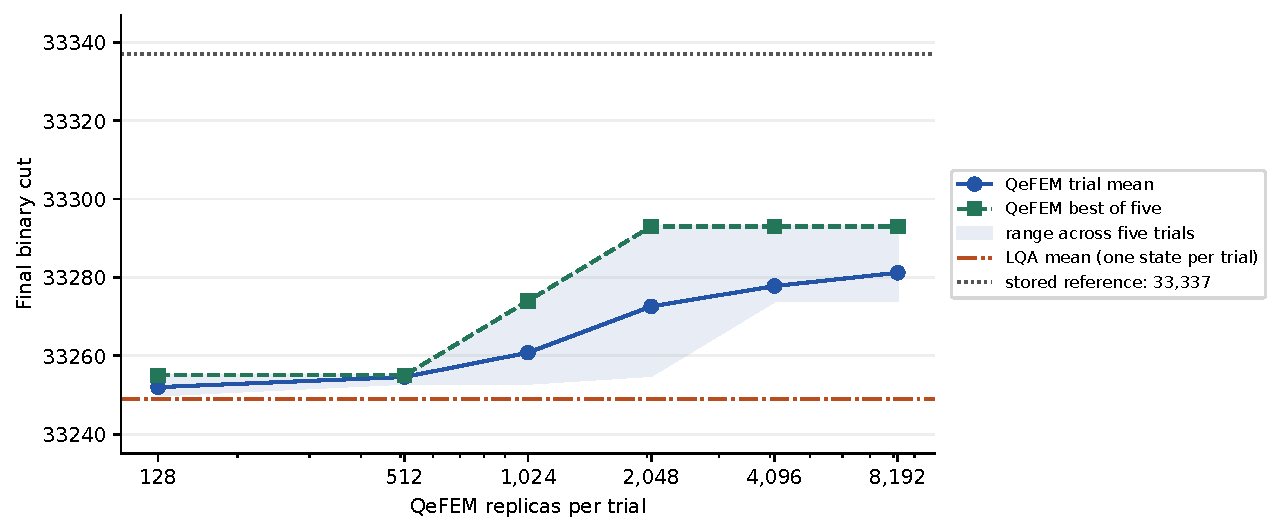
\includegraphics[width=.92\textwidth]{figures/k2000_population.pdf}
\caption{\textbf{Population search improves K2000 cut quality,
with diminishing best-cut returns.} QeFEM's mean, range, and best final
cut across five paired seeds are shown at each nested population size.
The saved \LQA{} mean (one state per trial) and the 33,337 stored target
are horizontal references. The best \QeFEM{} cut rises from 33,255
at 128 replicas to 33,293 by 2,048, then remains there through 8,192.
No point in this figure implies a matched-compute comparison.}
\label{fig:k2000-population}
\end{figure*}

The coherent final-winner trajectory in Fig.~\ref{fig:k2000-dynamics}
provides an additional view of the search. Its discrete reference gap
falls by orders of magnitude over the run, while local entropy per spin
decreases overall. The early entropy dip and rebound show that neither
entropy nor discrete cut changes monotonically under RMSprop and a
changing objective. The driver reaches zero halfway; the final portion
continues to refine the same candidate under a classical objective.
This selected trajectory illustrates a mechanism visible in one successful
trial; it does not describe the distribution of all 8,192 replicas.

\begin{figure*}[t]
\centering
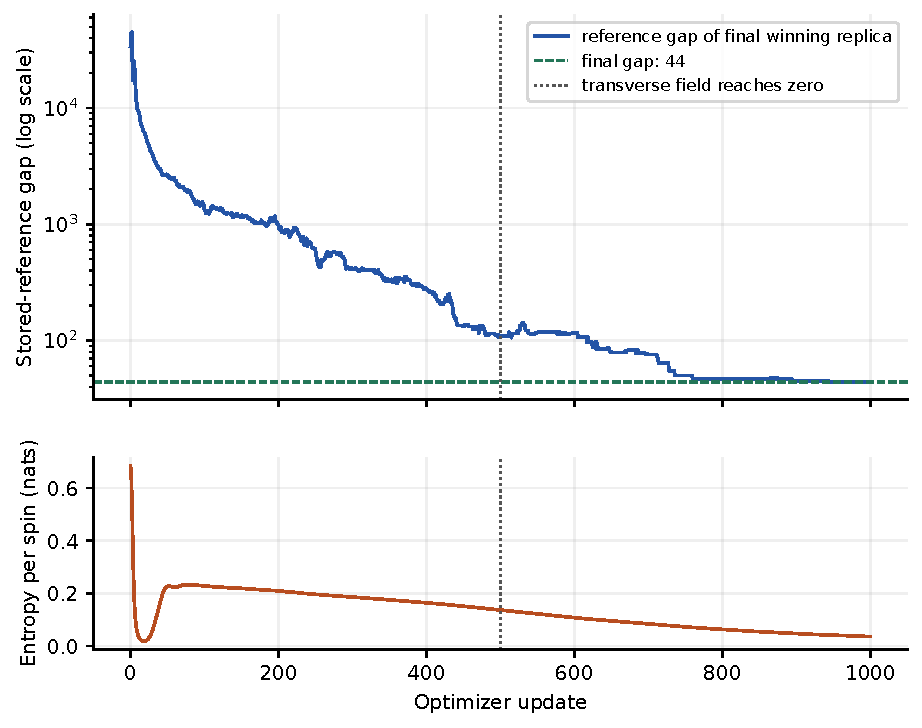
\includegraphics[width=.86\textwidth]{figures/k2000_winner_dynamics.pdf}
\caption{\textbf{Annealed mixed-state optimization can turn a
poor initialization into a near-reference binary solution.} The upper
panel shows the stored-reference gap on a logarithmic scale for one
coherent replica: the final winner of the best 8,192-replica K2000 trial.
The lower panel shows its mean single-site entropy. The dotted vertical
line marks the end of the transverse-field schedule; the dashed
horizontal line marks the final gap of 44. This is one replica's replay,
not a per-step maximum over the population.}
\label{fig:k2000-dynamics}
\end{figure*}

Taken together, the K2000 results support a specific and bounded claim.
The frozen mixed-state solver produces a high cut and improves on the
saved one-state \LQA{} baseline, but the explored population scaling
does not reach the reference. A new schedule or the G-set discrete update
might change that outcome; neither has been evaluated here and neither
can be credited for the frozen K2000 result.

\subsection{Wishart: lower error on every fixed planted instance}

The Wishart mean relative energy error is 4.0717\% for \QeFEM{} and
6.9411\% for the saved \LQA{} comparator. The difference is 2.8693
percentage points, or a 41.3\% reduction relative to the latter mean.
\QeFEM{} has lower mean error at each of the ten requested $\alpha$
values. Exact planted-energy hits occur in two of five trials at
$\alpha=0.9$ and all five at $\alpha=1.0$; the saved \LQA{} runs have
none across the 50 trials. The late improvement of \QeFEM{} after a
larger error at $\alpha=0.8$ is consistent with an easy--hard--easy
pattern in this particular ten-file series, but these fixed files alone
do not estimate an ensemble-wide hardness curve
\citep{hamze2020}.

\subsection{Chook: a wide planted-hit region}

Across the eleven tile-planted files, \QeFEM{} has equal-instance mean
relative error 0.2186\%; the saved \LQA{} mean is 1.1086\%. The
absolute difference is 0.8900 percentage points, corresponding to an
80.3\% relative reduction. \QeFEM{} has lower mean error on every file.
It reaches the planted energy in all ten trials for every requested
$p(C_3)$ from 0.5 through 1.0, accounting for 60 of 110 trial hits.
\LQA{} has four hits at 0.9 and six at 1.0, for ten of 110 overall.
The requested $p(C_3)$ is a generator setting; the realized tile
fraction of a finite instance can differ slightly.

\begin{figure*}[t]
\centering
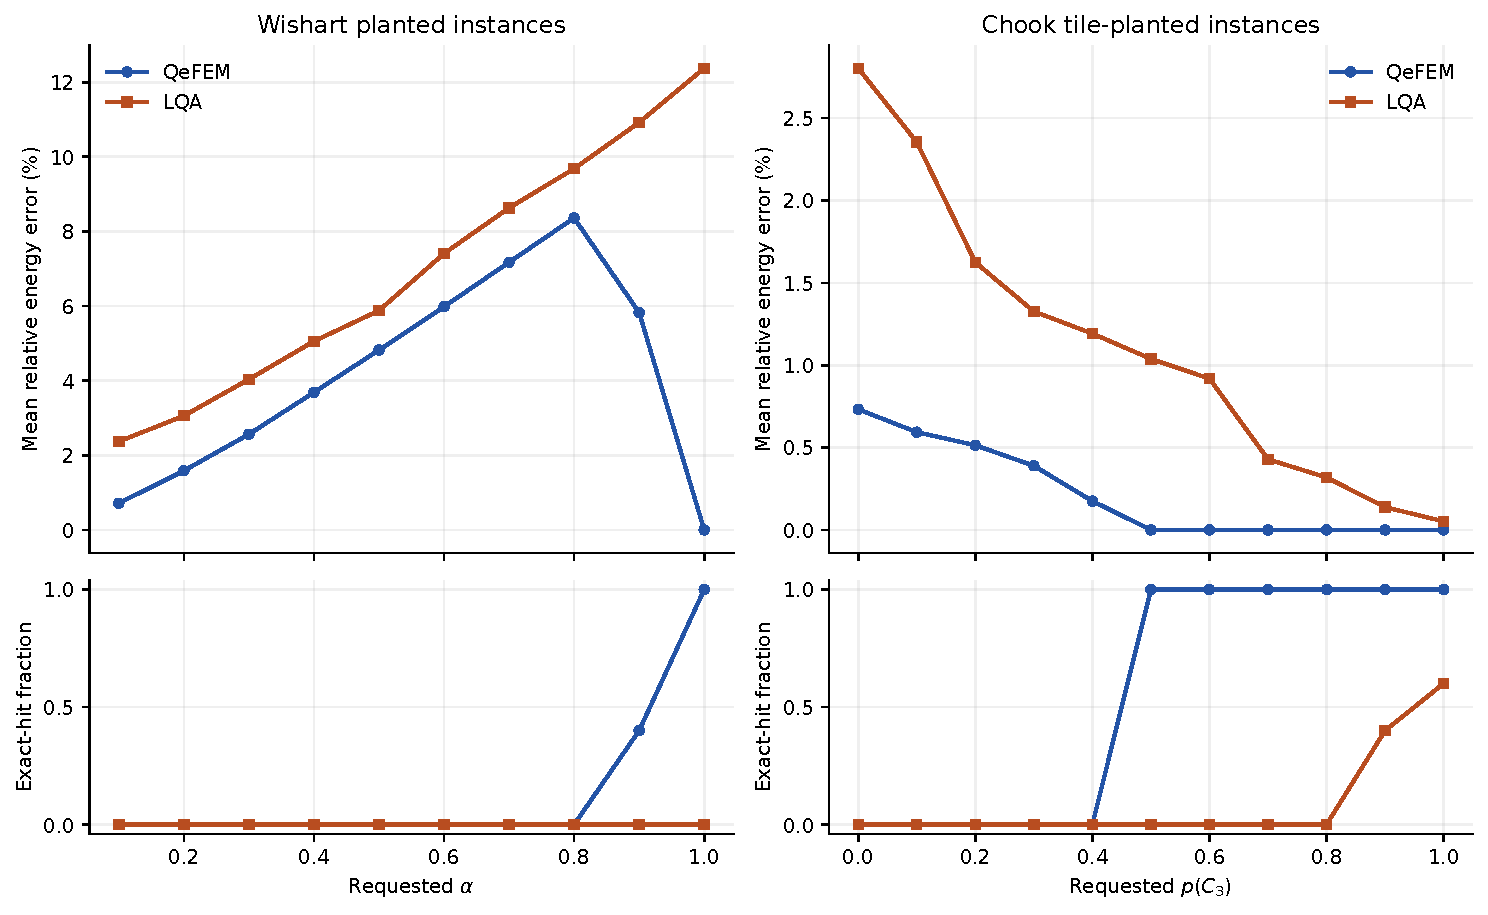
\includegraphics[width=\textwidth]{figures/planted_instance_errors.pdf}
\caption{\textbf{Under the saved configurations, \QeFEM{}
improves quality throughout both planted suites and reaches exact
solutions more often.} Top panels show trial-mean relative energy error
on each fixed Wishart and Chook instance. Bottom panels show the fraction
of trial populations whose best final replica has exactly the planted
energy. There are five trials per Wishart instance and ten per Chook
instance. The curves connect different fixed files and are visual guides,
not uncertainty bands or estimates over newly sampled instances.}
\label{fig:planted}
\end{figure*}

The two measures capture complementary outcomes. A lower mean error on
every file demonstrates consistent improvement over
the declared comparator, while exact hits distinguish a merely close
endpoint from a solved planted instance. The same plot also shows where
the gap has not closed: Wishart $\alpha\leq0.8$ yields no exact hit in
these five-seed batches.
